\chapter{Zielbestimmung}

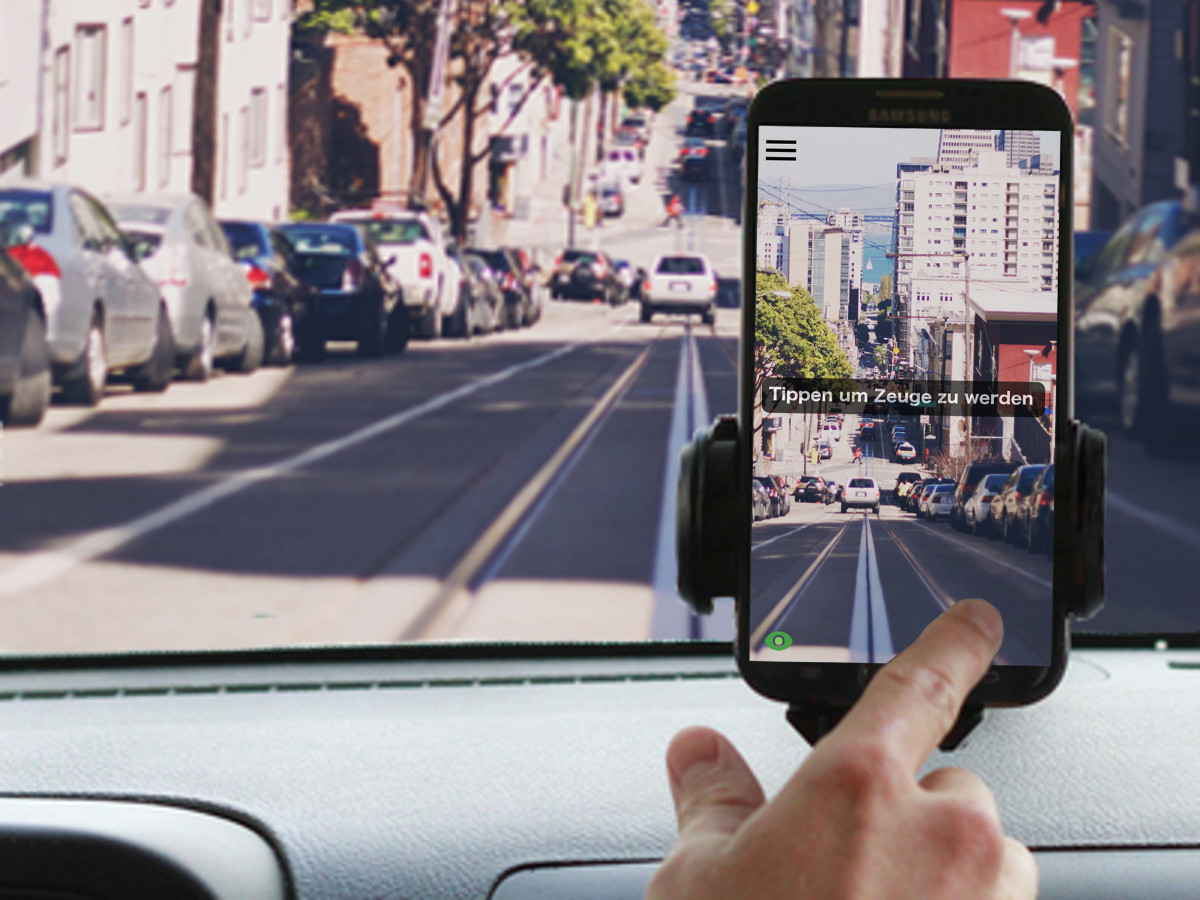
\includegraphics[width=\textwidth]{subtopicsFuncspec/Res//Mockups/Portrait_camera_view_car.jpg}\\[0.5cm]

Das Produkt ermöglicht es seinen Nutzern ihre Autofahrten zu überwachen, indem es durch die Handykamera den Straßenverkehr verfolgt und relevantes Videomaterial persistent abspeichert. Dieses wird bei Bedarf verwendet um einen Unfallhergang im Straßenverkehr zu dokumentieren. Dabei gilt es, dem deutschen Datenschutzrecht gerecht zu werden, indem Personen und personenbezogene Daten, wie zum Beispiel Autokennzeichen, unkenntlich gemacht werden.\newline
Zur Realisierung kann das Produkt in drei Hauptbestandteile aufgegliedert werden: Die Android App, den Webdienst und das Web-Interface. Diese Aufteilung wird in diesem Heft um Übersicht zu schaffen auch in nachfolgenden Kapiteln beibehalten und soll dem Nutzer eine moderne und intuitive Bedienoberfläche bieten.

\section{Musskriterien}
\subsection{App}
	\begin{enumerate}[\bfseries{PK}10]
	\setcounter{enumi}{99}
	\item Nutzer müssen sich einloggen um den Webdienst zu verwenden
	\item Nur registrierte Nutzer können die App verwenden
	\item Der Straßenverkehr wird durch die Handykamera beobachtet 
	\item Relevante Videodaten werden verschlüsselt abgespeichert
	\item Relevante Daten werden durch Auswertung der Sensordaten des Smartphones erkannt. Hierbei werden die Werte des G-Sensors ausgewertet
	\item Videodaten speichern relevante Metadaten
	\item Es wird ab dem Appstart mit dem Beobachten des Straßenverkehrs begonnen
	\item Es wird nur das Hochformat unterstützt
	\item Die Beobachtung läuft nur während sich die App im Vordergrund befindet
	\item Videodaten werden verschlüsselt, sobald sie persistiert werden
	\item Verschlüsselte Videodaten werden aufgelistet
	\item Verschlüsselte Videodaten können gelöscht werden
	\item Vom Nutzer ausgewählte verschlüsselte Videodaten werden an einen Webservice gesendet, der diese anonymisiert
	\item Geräte, auf denen Android API Level 19 (Android 4.4.4) und höhre läuft werden unterstützt
	\item Die Benutzeroberfläche wird für Geräte ab einer Displaydiagonale von 4 Zoll optimiert
	\item Wenn verschlüsselte Videodateien lange Zeit nicht zum anonymisieren ausgewählt wurden, wird der Nutzer benachrichtigt, dass er diese löschen kann
	\item Die aufnahmespezifischen Einstellungen werden angezeigt
	\item Die Standardsprache ist Deutsch
	\end{enumerate}
\subsection{Web-Dienst}
	\begin{enumerate}[\bfseries{PK}10]
	\setcounter{enumi}{199}
	\item Es existiert eine Schnittstelle, um Videodaten hochzuladen
	\item Von der App gesendete Videodaten werden anonymisiert
	\item Nach Abschluss der Anonymisierung wird der Nutzer per E-Mail benachrichtigt
	%\item Nach einer Registrierung bekommt der Nutzer eine Verifizierungs-E-Mail zugesendet
	\item Es existiert eine Schnittstelle, um Nutzeraccounts anzulegen
	\item Es existiert eine Schnittstelle, um Nutzeraccounts zu verwalten
	\item Es existiert eine Schnittstelle, um die Videodaten eines Nutzers verwalten zu können
	\item Nutzer müssen ihre E-Mail-Adresse verifizieren um sich einloggen zu können
	\item Die Kommunikation zwischen App und Webservice wird durch eine REST-API realisiert
	\item Die Kommunikation zwischen Web-Interface und Webservice wird durch eine REST-API realisiert
	\item Es existiert eine obere Schranke für die Anzahl der Videodateien, die ein Nutzer zur gleichen Zeit auf seinem Nutzeraccount online speichern kann
	\item Es wird Jetty verwendet
	\end{enumerate}
\subsection{Web-Interface}
	\begin{enumerate}[\bfseries{PK}10]
	\setcounter{enumi}{299}
	\item Es können Nutzeraccounts angelegt werden
	\item Es können Nutzeraccounts verwaltet werden
	\item Es können Videodaten verwaltet werden
	\item Es können Videodaten heruntergeladen werden
	\item Nur eingeloggte Nutzer haben Zugriff auf ihre Nutzerdaten
	\item Die Standardsprache ist Deutsch
	\end{enumerate}

\section{Wunschkriterien}
\subsection{APP}
	\begin{enumerate}[\bfseries{WK}10]
	\setcounter{enumi}{99}
	\item Falls es Android zulässt wird die Beobachtung auch ausgeführt, wenn sich die App im Hintergrund befindet
	\item Sowohl Quer- als auch Hochformat werden unterstützt
	\item Die Beobachtung kann manuell gestartet und gestoppt werden
	\item Die Aufnahme kann manuell gestartet werden, auch wenn die Sensoren des Smartphones keinen Anlass dazu geben
	\item Es können Nutzeraccounts angelegt werden
	\item Es können Nutzeraccounts verwaltet werden
	\item Anonymisierte Videodateien können vom Server gelöscht werden
	\item Push-Benachrichtignungen vom Web-Service werden angezeigt
	\item Es können Hilfestellungen für die Bedienung der App angezeigt werden
	\item Anonymisierte Videodateien können heruntergeladen werden
	\item Anonymisierte Videodateien die zum Download bereit stehen und sich nicht auf dem Smartphone befinden werden aufgelistet
	\item Anonymisierte Videodateien die sich auf dem Smartphone befinden  werden aufgelistet
	\item Anonymisierte Videodateien können vom Speicher des Smartphones gelöscht werden
	\item Anonymisierte Videodateien die sich auf dem Smartphone befinden können angesehen werden
	\item Die aufnahmespezifischen Einstellungen können bearbeitet werden
	\item So lange die Sensoren des Smartphones anlass zur Aufnahme geben wird weiter aufgenommen
	\end{enumerate}
\subsection{Web-Service}
	\begin{enumerate}[\bfseries{WK}10]
	\setcounter{enumi}{199}
	\item Die Zeit, die die Anonymisierung in Anspruch nehmen wird, wird geschätzt und and den Nutzer weitergeleitet
	\item Es wird eine Push-Benachrichtigung an das Smartphone gesendet, sobald die Anonymisierung der Videodaten abgeschlossen ist
	\item Videodaten werden maximal vier Wochen gespeichert
	\item Der Nutzer erhält eine Woche vor bevor ein Video glöscht wird eine E-Mail-Banchrichtigung
	\end{enumerate}
\subsection{Web-Interface}
	\begin{enumerate}[\bfseries{WK}10]
	\setcounter{enumi}{299}
	\item Das Produkt wird neuen Nutzern präsentiert
	\end{enumerate}

\section{Abgrenzungskriterien}
	\begin{enumerate}[\bfseries{AK}1010]
	\item Das betrachten nicht anonymisierter Videodaten ist nicht möglich
	\item Videodaten werden nicht automatisch persistiert sobald die Beobachtung läuft
	\item Livestreams werden nicht unterstützt
	\item Die Anonymisierung findet nicht auf dem Smartphone statt
	\item Der Web-Service speichert Videodaten nicht auf unbegrenzte Zeit und in unbegrenzter Anzahl
	\item Vom Speicher des Smartphones werden Videodaten nicht automatisch gelöscht
	\item Von Nutzern zurückgelegte Wege und besuchte Orte werden nicht aufgezeichnet
	\item Die App ist nicht mit Windows Phone und iOS kompatibel
	\item Die App wird nicht für Tablets optimiert
	\end{enumerate}